\documentclass[tikz,border=4pt]{standalone}
% Paleta y fuentes compartidas por el libro y las figuras (única fuente de verdad).
\RequirePackage{xcolor}
\definecolor{oxido}{HTML}{B7410E}
\definecolor{cobre}{HTML}{D27D2D}
\definecolor{carbon}{HTML}{2B2B2B}
\definecolor{azul}{HTML}{1F5F8B}
\definecolor{arena}{HTML}{F4EDE4}

\usepackage{fontspec}
\setsansfont{FiraSans}[Extension=.otf,UprightFont=*-Regular,BoldFont=*-SemiBold,ItalicFont=*-Italic,BoldItalicFont=*-SemiBoldItalic]
\usetikzlibrary{arrows.meta,calc,positioning,shapes.geometric}
\begin{document}
\sffamily\small
% Tres grados de certeza con los que el capítulo trata el futuro.
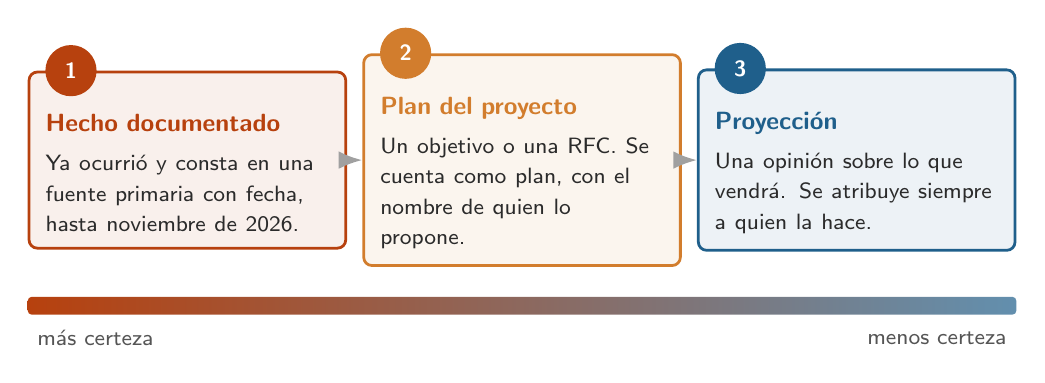
\begin{tikzpicture}[
  grado/.style={rounded corners=3pt,minimum height=17mm,text width=36mm,
    align=left,inner sep=6pt,font=\sffamily\small,
    execute at begin node={\hyphenpenalty=10000\raggedright}},
  etiq/.style={font=\sffamily\bfseries\footnotesize,text=white}]
  \foreach \n/\x/\c/\op/\t/\d in {
    1/0/oxido/1/Hecho documentado/{Ya ocurrió y consta en una fuente primaria con fecha, hasta noviembre de 2026.},
    2/4.25/cobre/0.85/Plan del proyecto/{Un objetivo o una RFC. Se cuenta como plan, con el nombre de quien lo propone.},
    3/8.5/azul/0.75/Proyección/{Una opinión sobre lo que vendrá. Se atribuye siempre a quien la hace.}}{
    \node[grado,draw=\c,line width=1pt,fill=\c!8] (g\n) at (\x,0) {%
      \rule{0pt}{5.5mm}{\bfseries\color{\c}\t}\\[3pt]{\footnotesize\color{carbon}\d}};
    \node[circle,fill=\c,minimum size=6.5mm,etiq] at ([xshift=5.5mm]g\n.north west) {\n};
  }
  \draw[-{Latex[length=3mm]},line width=1pt,carbon!45] (g1) -- (g2);
  \draw[-{Latex[length=3mm]},line width=1pt,carbon!45] (g2) -- (g3);
  % Barra de certeza: del óxido al azul, de más a menos certeza.
  \shade[left color=oxido,right color=azul!70,rounded corners=1.5pt]
    ($(g1.south west)+(0,-6mm)$) rectangle ($(g3.south east)+(0,-8mm)$);
  \node[anchor=north west,font=\sffamily\footnotesize,text=carbon!80]
    at ($(g1.south west)+(0,-9mm)$) {más certeza};
  \node[anchor=north east,font=\sffamily\footnotesize,text=carbon!80]
    at ($(g3.south east)+(0,-9mm)$) {menos certeza};
\end{tikzpicture}
\end{document}
